\documentclass{wissdoc}
%\documentclass[oneside]{wissdoc}
% ----------------------------------------------------------------
% Diplomarbeit - Hauptdokument
% ----------------------------------------------------------------
% wissdoc Optionen: draft, relaxed, pdf, oneside --> siehe wissdoc.cls
% ------------------------------------------------------------------
% Packages für Deckblatt
\usepackage[absolute]{textpos} 	%Textboxen an absolute Position setzen
\usepackage{setspace}						%Zeilenabstand anpassen
\usepackage{color}							%Farbige Schrift
\usepackage{graphicx}						%Einbinden von Grafiken

% Weitere packages: (Dokumentation dazu durch "latex <package>.dtx")
% \usepackage{varioref}
% \usepackage{verbatim}
% \usepackage{float}    %z.B. \floatstyle{ruled}\restylefloat{figure}
\usepackage{subfigure}
\usepackage[ngerman]{babel}
\usepackage[T1]{fontenc}
\usepackage[ansinew]{inputenc}
\usepackage{tabularx}

\usepackage{float}

% ----------------------------------------------------------------------
% used for code examples
\usepackage{listings}

\definecolor{lightgray}{rgb}{.9,.9,.9}
\definecolor{darkgray}{rgb}{.4,.4,.4}
\definecolor{purple}{rgb}{0.65, 0.12, 0.82}


\renewcommand\lstlistingname{Quelltext} % Change language of section name
\usepackage{xcolor}
\lstset{ % General setup for the package
	language=bash,
	basicstyle=\small\sffamily,
	backgroundcolor=\color{lightgray},
	numbers=left,
	numberstyle=\tiny,
	frame=tb,
	tabsize=4,
	columns=fixed,
	showstringspaces=false,
	showtabs=false,
	keepspaces,
	commentstyle=\color{red},
	keywordstyle=\color{blue}
}


\lstdefinelanguage{JavaScript}{
	keywords={typeof, new, true, false, catch, function, return, null, catch, switch, var, if, in, while, do, else, case, break},
	keywordstyle=\color{blue}\bfseries,
	ndkeywords={class, export, boolean, throw, implements, import, this},
	ndkeywordstyle=\color{darkgray}\bfseries,
	identifierstyle=\color{black},
	sensitive=false,
	comment=[l]{//},
	morecomment=[s]{/*}{*/},
	commentstyle=\color{purple}\ttfamily,
	stringstyle=\color{red}\ttfamily,
	morestring=[b]',
	morestring=[b]"
}

\lstset{
	language=JavaScript,
	backgroundcolor=\color{lightgray},
	extendedchars=true,
	basicstyle=\footnotesize\ttfamily,
	showstringspaces=false,
	showspaces=false,
	numbers=left,
	numberstyle=\footnotesize,
	numbersep=9pt,
	tabsize=2,
	breaklines=true,
	showtabs=false,
	captionpos=b
}
% ----------------------------------------------------------------------

% Zeilenabstand nach Vorgabe - Falls gefordert
%\setstretch{1,3} 

% Inhaltsangabe auf Unterabschnitte(2 Ebenen) begrenzen
\setcounter{tocdepth}{2}


% \usepackage{color}    % Farbiger/grauer Text
% \usepackage{colortbl}   % Farbige/graue Tabellenzeilen und -spalten!! <--
% \usepackage{fancybox} % für schattierte,ovale Boxen etc.
% \usepackage{tabularx} % automatische Spaltenbreite
% \usepackage{supertab} % mehrseitige Tabellen
%% ---------------- end of usepackages -------------

%% Informationen für die PDF-Datei
\hypersetup{pdfauthor={Max Mustermann},%
            pdftitle={Bachelorarbeit},%
            pdfsubject={Titel der Arbeit},%
            pdfkeywords={Forschung, Entwicklung, Funktechnik},%
            pdfproducer={LaTeX},%
            pdfcreator={pdfLaTeX}
}

% Macros, nicht unbedingt notwendig
%%%%%%%%%%%%%%%%%%%%%%%%%%%%%%%%%%%%%%%%%%%%%%%%%%%%%%%%%%
% macros.tex -- einige mehr oder weniger nuetzliche Makros
%%%%%%%%%%%%%%%%%%%%%%%%%%%%%%%%%%%%%%%%%%%%%%%%%%%%%%%%%%


%%%%%%%%%%%%%%%%%%%%%%%
% Kommentare 
%%%%%%%%%%%%%%%%%%%%%%%
\ifnotdraftelse{
\newcommand{\Kommentar}[1]{}
}{\newcommand{\Kommentar}[1]{{\em #1}}}
% Alles innerhalb von \Hide{} oder \ignore{} 
% wird von LaTeX komplett ignoriert (wie ein Kommentar)
\newcommand{\Hide}[1]{}
\let\ignore\Hide

%%%%%%%%%%%%%%%%%%%%%%%%%
% Leere Seite ohne Seitennummer, wird aber gezaehlt
%%%%%%%%%%%%%%%%%%%%%%%%%

\newcommand{\leereseite}{% Leerseite ohne Seitennummer, n�chste Seite rechts (wenn 2-seitig)
 \clearpage{\pagestyle{empty}\cleardoublepage}
}

%%%%%%%%%%%%%%%%%%%%%%%%%%
% Neue Seite rechts, leere linke Seite ohne Headings
%%%%%%%%%%%%%%%%%%%%%%%%%%
\newcommand{\xcleardoublepage}
{{\pagestyle{empty}\cleardoublepage}}

%%%%%%%%%%%%%%%%%%%%%%%%%%
% Tabellenspaltentypen (benoetigt colortbl)
%%%%%%%%%%%%%%%%%%%%%%%%%%
\newcommand{\PBS}[1]{\let\temp=\\#1\let\\=\temp}
\newcolumntype{y}{>{\PBS{\raggedright\hspace{0pt}}}p{1.35cm}}
\newcolumntype{z}{>{\PBS{\raggedright\hspace{0pt}}}p{2.5cm}}
\newcolumntype{q}{>{\PBS{\raggedright\hspace{0pt}}}p{6.5cm}}
\newcolumntype{g}{>{\columncolor[gray]{0.8}}c} % Grau
\newcolumntype{G}{>{\columncolor[gray]{0.9}}c} % helleres Grau

%%%%%%%%%%%%%%%%%%%%%%%%%%
% Anf�hrungszeichen oben und unten
%%%%%%%%%%%%%%%%%%%%%%%%%%
\newcommand{\anf}[1]{"`{#1}"'}

%%%%%%%%%%%%%%%%%%%%%%%%%%
% Tiefstellen von Text
%%%%%%%%%%%%%%%%%%%%%%%%%%
% S\tl{0} setzt die 0 unter das S (ohne Mathemodus!)
% zum Hochstellen gibt es uebrigens \textsuperscript
\makeatletter
\DeclareRobustCommand*\textlowerscript[1]{%
  \@textlowerscript{\selectfont#1}}
\def\@textlowerscript#1{%
  {\m@th\ensuremath{_{\mbox{\fontsize\sf@size\z@#1}}}}}
\let\tl\textlowerscript
\let\ts\textsuperscript
\makeatother

%%%%%%%%%%%%%%%%%%%%%%%%%%
% Gau�-Klammern
%%%%%%%%%%%%%%%%%%%%%%%%%%
\newcommand{\ceil}[1]{\lceil{#1}\rceil}
\newcommand{\floor}[1]{\lfloor{#1}\rfloor}

%%%%%%%%%%%%%%%%%%%%%%%%%%
% Average Operator (analog zu min, max)
%%%%%%%%%%%%%%%%%%%%%%%%%%
\def\avg{\mathop{\mathgroup\symoperators avg}}

%%%%%%%%%%%%%%%%%%%%%%%%%%
% Wortabk�rzungen
%%%%%%%%%%%%%%%%%%%%%%%%%%
\def\zB{z.\,B.\ }
\def\dh{d.\,h.\ }
\def\ua{u.\,a.\ }
\def\su{s.\,u.\ }
\newcommand{\bzw}{bzw.\ }

%%%%%%%%%%%%%%%%%%%%%%%%%%%%%%%%%%%
% Einbinden von Graphiken
%%%%%%%%%%%%%%%%%%%%%%%%%%%%%%%%%%%
% global scaling factor
\def\gsf{0.9}
%% Graphik, 
%% 3 Argumente: Datei, Label, Unterschrift
\newcommand{\Abbildung}[3]{%
\begin{figure}[tbh] %
\centerline{\scalebox{\gsf}{\includegraphics*{#1}}} %
\caption{#3} %
\label{#2} %
\end{figure} %
}
\let\Abb\Abbildung
%% Abbps
%% Graphik, skaliert, Angabe der Position
%% 5 Argumente: Position, Breite (0 bis 1.0), Datei, Label, Unterschrift
\newcommand{\Abbildungps}[5]{%
\begin{figure}[#1]%
\begin{center}
\scalebox{\gsf}{\includegraphics*[width=#2\textwidth]{#3}}%
\caption{#5}%
\label{#4}%
\end{center}
\end{figure}%
}
\let\Abbps\Abbildungps
%% Graphik, Angabe der Position, frei w�hlbares Argument f�r includegraphics
%% 5 Argumente: Position, Optionen, Datei, Label, Unterschrift
\newcommand{\Abbildungpf}[5]{%
\begin{figure}[#1]%
\begin{center}
\scalebox{\gsf}{\includegraphics*[#2]{#3}}%
\caption{#5}%
\label{#4}%
\end{center}
\end{figure}%
}
\let\Abbpf\Abbildungpf

%%
% Anmerkung: \resizebox{x}{y}{box} skaliert die box auf Breite x und H�he y,
%            ist x oder y ein !, dann wird das uspr�ngliche 
%            Seitenverh�ltnis beibehalten.
%            \rescalebox funktioniert �hnlich, nur das dort ein Faktor
%            statt einer Dimension angegeben wird.
%%
% \Abbps{Position}{Breite in Bruchteilen der Textbreite}{Dateiname}{Label}{Bildunterschrift}
%

\newcommand{\refAbb}[1]{%
s.~Abbildung \ref{#1}}

%%%%%%%%%%%%%%%%%%%%
%% end of macros.tex
%%%%%%%%%%%%%%%%%%%%

% Print URLs not in Typewriter Font
\def\UrlFont{\rm}

\newcommand{\blankpage}{% Leerseite ohne Seitennummer, nächste Seite rechts
 \clearpage{\pagestyle{empty}\cleardoublepage}
}

%% Einstellungen für das gesamte Dokument

% Trennhilfen
% Wichtig!
% Im german-paket sind zusätzlich folgende Trennhinweise enthalten:
% "- = zusätzliche Trennstelle
% "| = Vermeidung von Ligaturen und mögliche Trennung (bsp: Schaf"|fell)
% "~ = Bindestrich an dem keine Trennung erlaubt ist (bsp: bergauf und "~ab)
% "= = Bindestrich bei dem Worte vor und dahinter getrennt werden dürfen
% "" = Trennstelle ohne Erzeugung eines Trennstrichs (bsp: und/""oder)

% Trennhinweise fuer Woerter hier beschreiben
\hyphenation{
% Pro-to-koll-in-stan-zen
% Ma-na-ge-ment  Netz-werk-ele-men-ten
% Netz-werk Netz-werk-re-ser-vie-rung
% Netz-werk-adap-ter Fein-ju-stier-ung
% Da-ten-strom-spe-zi-fi-ka-tion Pa-ket-rumpf
% Kon-troll-in-stanz
}

%Tabellen Kommandos
\newcolumntype{L}[1]{>{\raggedright\arraybackslash}p{#1}}
\newcolumntype{C}[1]{>{\centering\arraybackslash}p{#1}}
\newcolumntype{R}[1]{>{\raggedleft\arraybackslash}p{#1}}

% Index-Datei öffnen
\ifnotdraft{\makeindex}
%%%%%%%%%%%%%% includeonly %%%%%%%%%%%%%%%%%%%
% Es werden nur die Teile eingebunden, die hier aufgefuehrt sind!
%\includeonly{%
%titelseite,%
%erklaerung,%
%kurzfassung,%
%einleitung,%
%analyse,%
%entwurf,%
%implemen,%
%zusammenf%
%}
%%%%%%%%%%%%%%%%%%%%%%%%%%%%%%%%%%%%%%%%%%%%%%
\begin{document}
%Auskommentiert, da nicht notwendig für das Praktikum
%\ifnotdraft{
	%%%%Vorlage
	% 
\thispagestyle{empty}
\begin{figure}[t]
		\hspace{-2.2cm}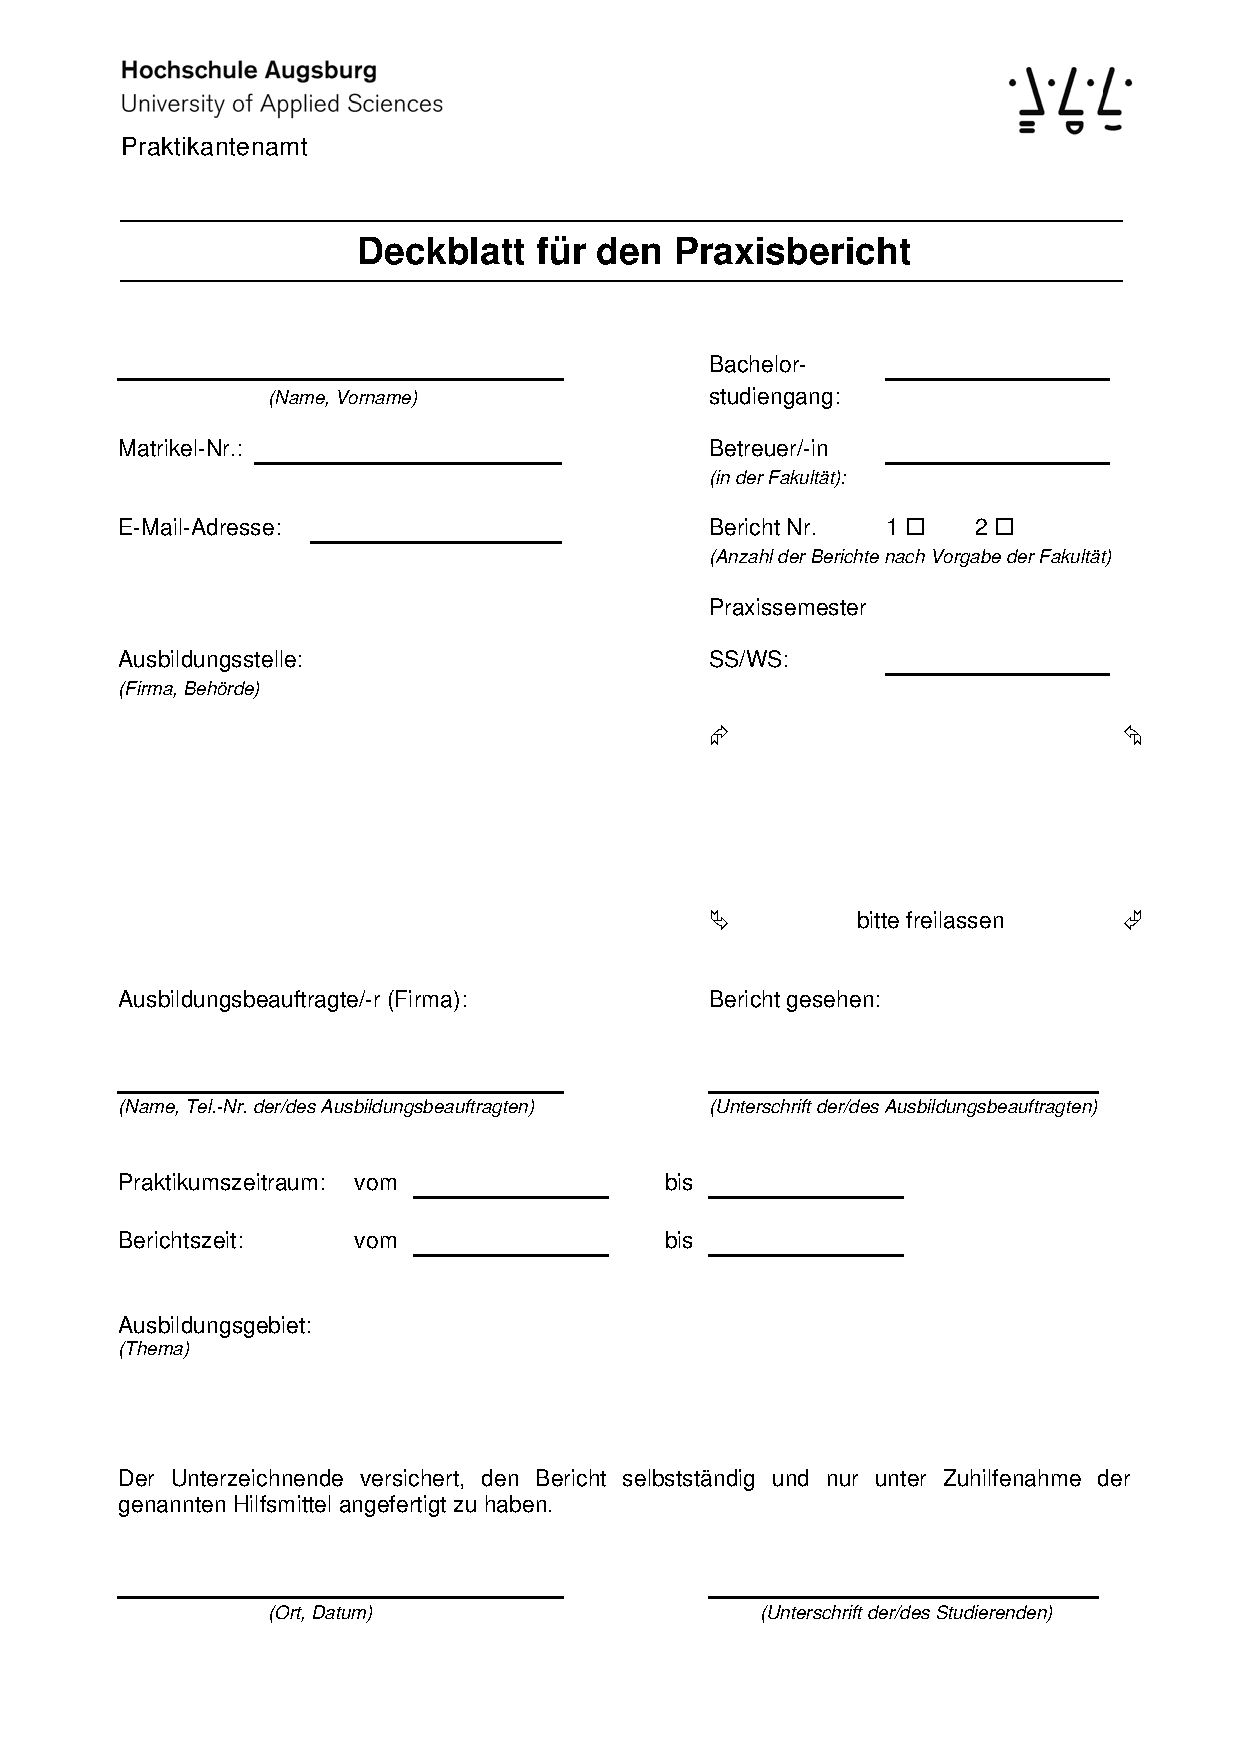
\includegraphics[width=0.93\paperwidth]{figures/deckblatt_prax_bac}
	\label{fig:deckblatt_prax_bac}
\end{figure}
  %<-- Nach Vorgabe der HS Augsburg

	%%% Deckblatt - Hochschule Augsburg
%%%Deckblatt

\textblockorigin{20mm}{30mm}

\thispagestyle{empty}\null
%%%%Logo - Hochschule Augsburg - Informatik
\begin{textblock}{10}(8.0,1.1)
\begin{figure}[h]
	\centering
		
\includegraphics[width=0.45\textwidth]{logos/hsa_informatik_logo_lq.pdf}
\end{figure}

\end{textblock}

%%% Text unter Logo
\begin{textblock}{15}(12.43,2.1)
	\LARGE
	\textsf{
		\textbf{\textcolor[rgb]{1,0.41,0.13}{\\
			\begin{flushleft}
				Fakult�t f�r\\
				Informatik\\
			\end{flushleft}
			}
		}
	}
\end{textblock}

%%%%Textbox links - Informationen
\begin{textblock}{15}(2,1.4)
	%\LARGE
	\begin{flushleft}
		\begin{spacing} {1.2}
			\huge	
				\textbf{Methoden der KI\\}
				\vspace{30pt}
				\textcolor[rgb]{1,0.41,0.13}{\\
				\textbf{Portfoliopr�fung}}\\
				\vspace{60pt}
			\LARGE
				Studienrichtung\\
				Technische Informatik\\
				\vspace{40pt}
				
				Muhammad Aman Bin Ahmad Tifli\\
				\vspace{30pt}		
				Matrikelnummer: 2042550\\
				% \vspace{30pt}		
				% Ausbildungsstelle: KUKA Deutschland AG\\
				\vspace{60pt}		
			\LARGE
				Pr\"ufer: Prof. Dr. Thomas Rist\\
				\vspace{10pt}		
				Abgabedatum: xx.xx.2021\\
			\end{spacing}
		\end{flushleft}
		
\end{textblock}



%%%%Textbox rechts - Hochschule
\begin{textblock}{5}(12.45,9.0)
	\scriptsize
	\textcolor[rgb]{1,0,0}{\\
		\begin{flushleft}
			\begin{spacing} {1.3}
				Hochschule f\"ur angewandte\\
				Wissenschaften Augsburg\\
				\vspace{4pt}
				An der Hochschule 1\\
				D-86161 Augsburg\\
				\vspace{4pt}
				Telefon +49 821 55 86-0\\
				Fax +49 821 55 86-3222\\
				www.hs-augsburg.de\\
				info(at)hs-augsburg-de
			\end{spacing}
		\end{flushleft}
		}
\end{textblock}


%%%%Textbox rechts unten - Fakult?t und Autor
\begin{textblock}{5}(12.45,11.5)
	\scriptsize
		\begin{flushleft}
			\begin{spacing} {1.3}
				Fakult\"at f\"ur Informatik\\
				Telefon +49 821 55 86-3450\\
				Fax \hspace{10pt} +49 821 55 86-3499\\
				\vspace{6pt}
				Verfasser der Diplomarbeit\\
				Max Mustermann\\
				Beispielstra?e 31\\
				86150 Augsburg\\
				Telefon +49 821 55 86-3450\\
				max@hs-augsburg.de\\
			\end{spacing}
		\end{flushleft}
	\end{textblock}
\pagebreak  %<-- Nach Vorgabe der HS Augsburg
	%
	%%%% Innere Titelseite 
 	%\include{titelseite} %<-- Vorgabe Prüfer oder frei wählbar
	%
	%%%%Optional - Falls von der Firma gefordert
	%\include{sperrvermerk}
	%
	%%%%Pflicht
 	%\include{erklaerung}
	%
	%%% Leere Seite bei zweiseitigem Druck
	%\ifnotonesideelse{\blankpage}{}
	%\include{kurzfassung}
	%%% Leere Seite bei zweiseitigem Druck
	%\ifnotonesideelse{\blankpage}{}
%}



%
%% ++++++++++++++++++++++++++++++++++++++++++
%% Verzeichnisse
%% ++++++++++++++++++++++++++++++++++++++++++
\pagenumbering{roman}
\ifnotdraft{
\tableofcontents
% Leere Seite bei zweiseitigem Druck
%\ifnotonesideelse{\blankpage}{}
%\listoffigures
%% Leere Seite bei zweiseitigem Druck
%\ifnotonesideelse{\blankpage}{}
%\listoftables
%% Leere Seite bei zweiseitigem Druck
%\ifnotonesideelse{\blankpage}{}
}
%% ++++++++++++++++++++++++++++++++++++++++++
%% Hauptteil
%% ++++++++++++++++++++++++++++++++++++++++++
\graphicspath{{figures/}}
\pagenumbering{arabic}

%%% Ab hier eigene Kapitel einfügen
%%% Kapitel sind analog zur Wordvorlage zu wählen

\chapter{Introduction}
\chapter{Formulierung von Problemen und Lösungen in der Symbolischen Informationsverarbeitung}
\chapter{Probleml�sung als Suchaufgabe}

\section{Wegsuche ohne Karte}

``Wegsuche ohne Karte'' bedeutet Wegfindung in einer unbekannten Umgebung ohne eine Karte, die den Agenten leitet.

Beispiel: \textbf{Roboter R} befindet sich in einem unbekannten Gebiet und muss sich zu einem Zielobjekt bewegen. Dies kann durch Anwendung eines \textbf{Bug-Algorithmus} gel�st werden, der voraussetzt, dass der Roboter mit Sensoren ausgestattet ist, um Hindernisse und das \textbf{Zielobjekt S} zu erkennen.

\subsection{Bug Algorithmen Beispiel}
\label{bug-algo-1}
Ein Beispiel f�r einen Bug-Algorithmus ist wie folgt:
\begin{enumerate}
    \item Wenn das \textbf{Zielobjekt S} in Sichtweite ist, fahrt \textbf{Roboter R} direkt darauf zu
    \item Wenn \textbf{S} nicht in Sicht ist, aber stattdessen ein Hindernis vorhanden ist, bewegt sich \textbf{R} gem�� einer bestimmten Regel um das Hindernis herum (z. B. im Uhrzeigersinn).
    \item \textbf{R} scannt erneut nach dem Objekt \textbf{S} und wiederholt die Schritte 1 und 2, bis das Ziel erreicht ist.
\end{enumerate}

\begin{figure}[H]
    \centering
    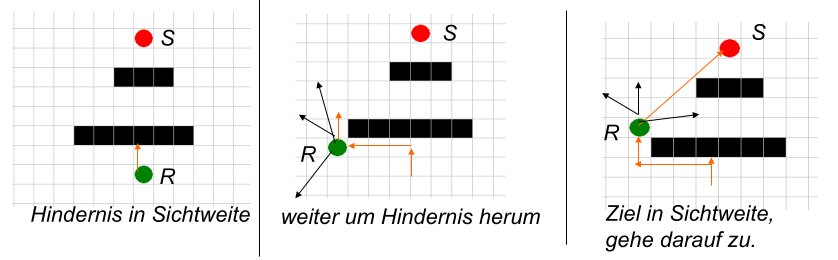
\includegraphics[width=\textwidth]{figures/kap3/bug-algo-1.png}
    \caption{Beispiel von Bug-Algorithmus Verfahren}
    \label{fig:bug-algo}
\end{figure}

\subsection{Problem mit dem Bug-Algorithmus}

In bestimmten Situationen (z.B siehe Abb. \ref{fig:bug-algo-prob}) ist der Roboter mit dem Ansatz in Abschnitt~\ref{bug-algo-1} nicht in der Lage, das Ziel zu finden.

\begin{figure}[H]
    \centering
    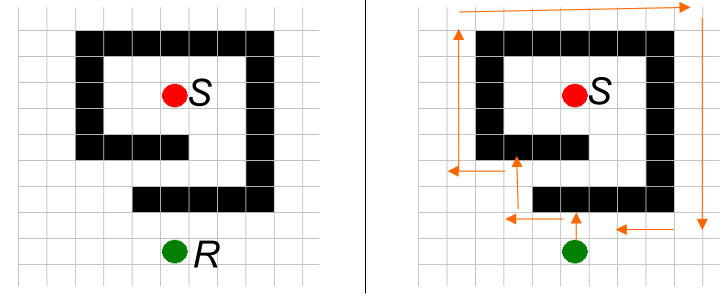
\includegraphics[width=0.8\textwidth]{figures/kap3/bug-algo-1-problem.png}
    \caption{Der Roboter kann das Ziel nicht sehen}
    \label{fig:bug-algo-prob}
\end{figure}

Der Algorithmus muss verbessert werden, z. B. durch Bewegen gegen den Uhrzeigersinn, um eine Bewegung in einem kontinuierlichen Kreis zu vermeiden.

\begin{figure}[H]
    \centering
    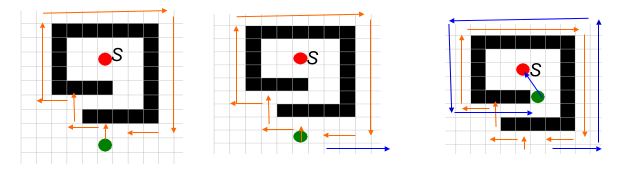
\includegraphics[width=\textwidth]{figures/kap3/bug-algo-1-fix.png}
    \caption{Gegen den Uhrzeigersinn bewegen, um das Ziel zu erreichen}
    \label{fig:bug-algo-fix}
\end{figure}

\section{Repr�sentation von Suchr�umen}

\subsection{Suchraum als Karte}

Ein Suchraum wird normalerweise als grafische Karte dargestellt. Diese Karten k�nnen als Wegenetz oder als Gitter mit benachbarten Zellen dargestellt werden, wie in Abbildung \ref{fig:graph-examples} gezeigt.

\begin{figure}[H]
    \centering
    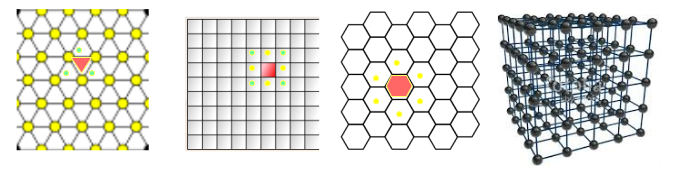
\includegraphics[width=\textwidth]{figures/kap3/graph-examples.png}
    \caption{Beispiele von Gittermustern}
    \label{fig:graph-examples}
\end{figure}

Je nach verwendetem Gittermuster werden unterschiedliche Suchgraphen basierend auf der Anzahl der Nachbarn jeder Zelle im Gitter gebildet. Zum Beispiel: Eine dreieckige Zelle hat sechs Nachbarn, eine quadratische Zelle hat 4 (oder 8, wenn Diagonalen erlaubt sind) und eine sechseckige Zelle hat 6.

\section{Wegsuche als systemstisches Ablaufen von Graphen}

Bei der Wegfindung mit Hilfe eines Graphen m�ssen ein \textbf{Startknoten} und eine \textbf{Funktion zum Testen}, ob der Zielknoten erreicht wurde, definiert werden. Mit Hilfe des Startknotens und dieser Funktion kann eine Folge von Knoten gefunden werden, die die Testfunktion erf�llen k�nnen. Wichtig ist, dass die f�r die Sequenz ausgew�hlten Knoten \textbf{benachbarte Knoten sind, die durch Kanten verbunden} sind.

\subsection{Expliziter Graphen und sukzessive Expansion}

Es ist wichtig, zwischen einem expliziten Graphen und einem ``gedachten'' Graphen als Repr�sentation eines Suchraums f�r L�sungen zu unterscheiden.

\paragraph{Expliziter Graphen}

Eine explizite Darstellung der Knoten und Kanten ist verf�gbar (z.B Adjazentmatrix). Dies ist nur f�r kleinere Knotenmengen praktikabel und die meisten Probleme erfordern keine vollst�ndige Repr�sentation des Suchgraphen.

\paragraph{Sukzessive Expansion}

Diagramm ist verf�gbar, aber nicht vollst�ndig explizit. Der Suchprozess erfolgt durch Knotenerweiterung, indem Knoten f�r Knoten vorgegangen wird.

\subsection{Generelle Wegfindungsstrategie}

Zyklen und Mehrfachbesuche sind zu vermeiden, da sie den Suchbaum exponentiell wachsen lassen k�nnen. Generell sollte man keinen bereits benutzten Weg nochmal gehen, keine Wege mit Zyklen kreieren, einen bereits besuchten oder ausgebauten Zustand nicht nochmal besuchen oder erzeugen.

\subsection{Generelle Bewertung von S uchverfahren} 

Bewertungskriterien eines Pfadfindungsprozesses sind wie folgt:

\paragraph{Korrektheit}

Es ist wichtig, dass die Wegfindungsl�sung tats�chlich eine L�sung des Problems ist.

\paragraph{Vollst�ndigkeit}

Existiert eine L�sung, terminiert der Algorithmus nach endlicher Zeit und generiert eine L�sung.

\paragraph{Optimalit�t}

Die optimalste L�sung wird gefunden, wenn mehrere m�glich sind.

\paragraph{Zeitkomplexit�t}

Die Zeit, die im worst-case/average-case ben�tigt wird, um eine optimale L�sung zu finden.

\paragraph{Speicherkomplexit�t}

Wie viel Speicher, die im worst-case/average-case ben�tigt wird.



\section{Arten von Suchverfahren}

Es gibt viele M�glichkeiten, eine Wegfindungssuche durchzuf�hren. Diese n�chsten Abschnitte werden darauf eingehen.

\subsection{Breitensuche in expliziten Graphen}
\label{section:breitensuche}
Breitensuche ist auf Englisch ``breadth first search''. F�r diesen Algorithmus werden f�r jeden Knoten zus�tzliche Daten ben�tigt: \textbf{noch nicht gesucht} (wei� dargestellt), \textbf{entdeckt, aber noch nicht verarbeitet } (grau dargestellt), \textbf{verarbeitet} (schwarz dargestellt). 

\paragraph{�berblick �ber den Ablauf:}

\begin{enumerate}
    \item W�hle einen Startknoten aus dem Graphen und legen Sie diesen in die Warteschlange, Q. Alle Knoten in Q sind grau markiert.
    \item Solange es Elemente in Q gibt, markiere alle Nachbarn der Elemente grau und f�ge diese der Warteschlange Q hinzu. 
    \item Nachdem alle Nachfolger eines Knotens grau markiert wurden, markiere den Knoten schwarz und entferne ihn aus der Warteschlange. Pr�fen Sie, w�hrend Sie die Nachfolgerknoten grau markieren, ob der zu markierende Knoten der Zielknoten ist.s
    \item Wiederhole Schritt 2 und Schritt 3, bis die Warteschlange Q leer ist.
\end{enumerate}

\paragraph{Komplexit�tsbetrachtung}

Speicherbedarf und Zeitbedarf sind exponentiell. Dies f�hrt dazu, dass gro�e Graphen unl�sbar sind und sogar relativ kleine Graphen zu lange brauchen, um praktikabel zu sein (z.B Graphen Tiefe 12 brauch 35 Jahre Rechenzeit).

\subsection{Uniforme Kostensuche}

Bei diesem Suchalgorithmus wird die Breitensuche so ver�ndert, dass auch die \textbf{Kosten der Nachbarknoten} ber�cksichtigt werden. Da die Kosten zweier benachbarter Knoten normalerweise bereits bekannt sind, kann \textbf{die Warteschlange in einen Heap umstrukturiert werden}, der in \textbf{aufsteigender Reihenfolge der Pfadkosten} sortiert ist. Auf diese Weise wird gehofft, dass der k�rzeste Weg vom Startknoten zum Zielknoten gefunden wird.

\subsection{Modifizierte Uniforme Kostensuche / Dijkstra}

Um eine optimale L�sung f�r ein Wegsucheproblem zu finden, ist es notwendig, alternative Pfade parallel zu konstruieren. Wenn sich diese Pfade am selben Punkt treffen, kann der \textbf{k�rzeste Pfad beibehalten werden}, w�hrend der Rest aus dem Suchbaum entfernt wird, um die k�rzeste Gesamtroute zu finden.

Wenn ein Pfad zum Zielknoten gefunden wird, werden alle \textbf{anderen parallelen Pfade fortgesetzt}, es sei denn, ihre Kosten �bersteigen den bereits gefundenen Pfad. Dies f�hrt zu einer besseren Effizienz bei der Suche nach dem k�rzesten Weg. 

\begin{figure}[H]
    \centering
    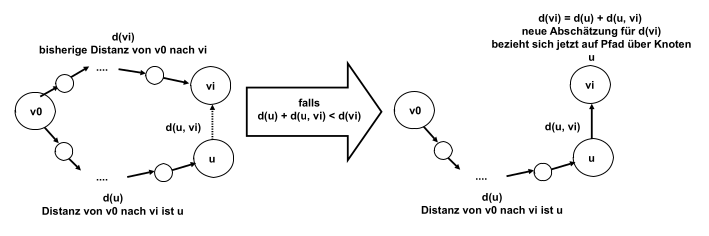
\includegraphics[width=\textwidth]{figures/kap3/dijkstra.png}
    \caption{Dijkstra-Algorithmus Pfadsuche}
    \label{fig:graph-dijkstra}
\end{figure}

Dieser Algorithmus ist in Abbildung \ref{fig:graph-dijkstra} demonstriert. Anhand der Abbildung kann man sehen, wie die beiden Routen von v0 nach vi verglichen werden und die Kosten verglichen werden, um nur die k�rzere Route beizubehalten.

\subsection{Ablauf eines Graphen mit Tiefensuche}

Im Gegensatz zur Traversierung mit Breitensuche verl�uft die Traversierung mit Tiefensuche auf m�glichst langen Wegen und f�hrt die Wei�-Grau-Schwarz-Markierung (siehe Abschnitt \ref{section:breitensuche}) durch. Dieser Algorithmus wird normalerweise rekursiv implementiert.

\paragraph{Ablauf von Tiefensuche}

\begin{enumerate}
    \item W�hle einen Startknoten \( v_s \). Markiere den Knoten als grau ein.
    \item F�r jeden Nachbarknoten \( v_k \) von \( v_s \), der wei� markiert ist, f�hre folgendes durch:
    \begin{enumerate}
        \item F�ge \( v_k \) zum Stack hinzu
        \item Markiere \( v_k \) als grau
        \item Falls \( v_k \) Nachbarn hat, f�hre Schritt (2) rekursiv aus
        \item Wenn \( v_k \) keine Nachbarn hat oder seine Nachbarn schwarz markiert sind, markiere \( v_k \) schwarz und entferne \( v_k \) vom Stack
    \end{enumerate}
    \item Der Algorithmus endet, sobald der Stack leer ist.
\end{enumerate}

\paragraph{Komplexit�tsbetrachtung}

Nur benachbarte Knoten des aktuellen Suchpfads werden auf dem Stack gespeichert. Dies bedeutet viel weniger Knotenerweiterungen im Vergleich zur Breitensuche, was zu weniger Speicherverbrauch f�hrt. Die Zeitkomplexit�t ist jedoch ebenso wie die Brreitensuche exponentiell.

\subsection{Tiefensuche und Backtracking-Algorithmen}

In realen Anwendungen beinhaltet eine L�sung die Verwendung vieler verschiedener Komponenten. Die endg�ltige L�sung verwendet daher normalerweise viele Teill�sungen, die m�glicherweise nicht richtig erweitert werden k�nnen (z.B: erreicht die Teill�sung eine Sackgasse). In diesen F�llen muss die Teill�sung durch eine weniger komplexe L�sung ersetzt werden.

\paragraph{Genereller Ablauf von einem Backtracking-Algorithmus}

Gegeben sind ein Array ``SolutionComponents'', das alle Werte der endg�ltigen L�sung enth�lt, und die Funktionen ``FirstTrialValue()'', ``NextTrialValue()'' und ``CheckValid()''.

\begin{enumerate}
    \item Der ersten Komponente wird der erste Versuchswert gegeben:\\~\\
    \lstinline{SolutionComponents[0] = FirstTrialValue(0)}~\\
    \item Die G�ltigkeit der L�sung wird �berpr�ft:\\~\\
    \lstinline{CheckValid(SolutionComponents)}~\\
    \item Wenn die bisherige L�sung g�ltig ist, fahren Sie mit dem n�chsten Wert fort (i = 1, 2, 3...) und �berpr�fe den Wert erneut\\~\\
    \lstinline{SolutionComponents[i] = FirstTrialValue(i)}~\\
    \lstinline{CheckValid(SolutionComponents)}~\\
    \item Wenn der CheckValid-Funktion an einem bestimmten Punkt false zur�ckgibt, versuche es mit den n�chsten Werten. Wenn alle Werte ebenfalls falsch zur�ckgeben, f�hre ein Backtracking durch, indem Sie i um i reduzieren und den n�chsten Wert f�r dieses i versuchen.Erh�hen Sie dann i wieder um 1 und probieren Sie alle Werte aus.
    \item Schritt 4 wird so oft wie n�tig wiederholt. F�r den Fall, dass i null erreicht und es keine Versuchswerte mehr f�r i = 0 gibt, gibt es keine m�gliche L�sung.
\end{enumerate}

\subsection{Limitierte Tiefensuche}

Es ist m�glich, die Nachteile der Tiefensuche zu vermeiden, indem man eine maximale Tiefe des Pfades einstellt. Das macht die Suche vollst�dnig aber nicht immer optimal. Um diese Idee zu erweitern, kann eine iterative Tiefensuche versucht werden. 

\subsection{Iterative Tiefensuche}

Bei dieser Methode wird die Tiefe mit jeder Iteration erh�ht, um sicherzugehen, dass eine L�sung gefunden wird.

\subsection{Bidirektionale Suche}

Anstatt nur vom Startknoten aus zu beginnen, f�hren Sie eine Suche vom Start- und vom Zielknoten aus durch. Wenn sich die beiden Verfahren in der Mitte treffen, ist eine L�sung gefunden.

\section{KI-Suchverfahren}

Es gibt zwei Klassen von Suchverfahren: \textbf{blinde Suchverfahren} und \textbf{KI-Suchverfahren}. Blinde Suchverfahren sind auf einem bestimmten Schema basiert, das unabh�ngig von dem jeweiligen Problem ist. Einige Beispiele hierf�r sind die in den vorangegangenen Kapiteln behandelten Verfahren wie Breitensuche, Tiefensuche, Biridketionale Suche usw. 

KI-Suchverfahren hingegen nutzen problemspezifisches Vorwissen zur Eingrenzung des Suchraums. Es handelt sich um informierte heuristische Suchverfarhen.

\textbf{Blinde Suchverfahren} erfordern, dass eine L�sung durch systematische und ersch�pfende Suche in einem Suchgraphen gefunden wird, was ineffizient und kein problemspezifisches Wissen nutzt.

\textbf{Informierte Suchprozesse} hingegen nutzen problemspezifische Eigenschaften, um die Effizienz der Knotenexpansion zu verbessern.

\subsection{Greedy Search}
\label{section:greedy-search}
Die Greedy-Suche ist eine modifizierte Breitensuche (siehe Abschnitt \ref{section:breitensuche}), bei der nur die Knoten mit den geringsten Kosten in die Warteschlange aufgenommen werden. 

\paragraph{Ablauf von Greedy Search}

Wenn die Kosten des aktuellen Knotens zum Zielknoten unbekannt sind, \textbf{m�ssen diese Kosten gesch�tzt werden}, und dann wird der Nachbar mit den geringsten Kosten ausgew�hlt. Die Funktion, die diese Kosten sch�tzt, wird \textbf{heuristische Funktion} genannt.

Der Unterschied zwischen Greedy Search und Uniform Cost Search (siehe Abschnitt \ref{section:uniform-cost-search}) besteht darin, dass bei der Greedy Search \textbf{die Kosten von einem Knoten zum Zielknoten} berechnet werden und nicht von einem Knoten zum anderen.

\paragraph{Eigenschaften von Greedy Search}

Greedy Search bietet tendenziell schnelle L�sungen, die oft, aber nicht immer, der optimale Weg sind. 

Greedy Search ist �hnlich wie die Tiefensuche mit Backtracking, nicht vollst�ndig, und erfordert eine gute Heuristik f�r eine bessere G�te des Verfahrens.

\subsection{Der A* Algorithmus}

Der A*-Algorithmus ist ein neuer Ansatz, der auf Greedy Search (Abbschnitt~\ref{section:greedy-search}) und dem Dijkstra-Algorithmus~(Abbschnitt~\ref{section:dijkstra}) aufbaut. A* arbeitet basierend auf der Funktion:

\[f(n) = g(n) + h(n)\]

Wobie \(f(n)\) die gesch�tzten Kosten der billigsten L�sung ist, \(g(n)\) die Kosten f�r die Bewegung von der Ausgangszelle zur aktuellen Zelle, und \(h(n)\) die gesch�tzten Kosten f�r die Bewegung von der aktuellen Zelle zur Zielzelle. Mit der Funktion \(f(n)\) werden die Kosten berechnet, und der Rest des Algorithmus l�uft wie bei Greedy Serach ab.

\subsection{Pfadplannung mit A*}

\subsection{Pfadplannung in Computerspielen}



\section{Vertiefungsprojekt: A*-Pfadfindung}

Um besser zu verstehen, wie die A*-Pfadfindung funktioniert (und um etwas Spa� beim Programmieren zu haben), wurde der Algorithmus in Java implementiert. Diese Umsetzung basiert auf einem Online-Artikel von Baeldung\cite{a-star-online}. Die Struktur des Gesamtprojekts und seine Durchf�hrung werden in Kapitel \ref{section:vertiefungs-projekt} erl�utert. 

\begin{figure}[H]
    \centering
    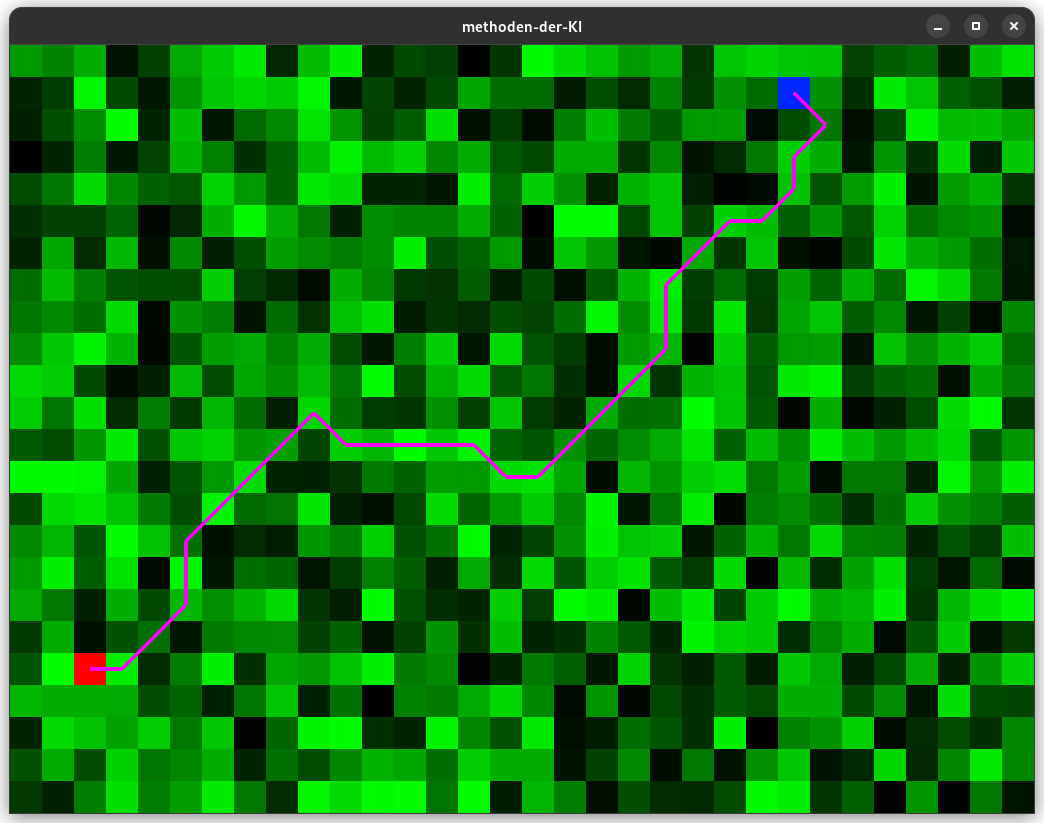
\includegraphics[width=\textwidth]{figures/kap3/a-star-impl.png}
    \caption{Der A*-Pfadfindungs-Screen}
    \label{fig:impl-a-star-pathfinding}
\end{figure}

Bei der Umsetzung wird ein zuf�lliges Terrain in Form von gr�nen Quadraten erzeugt. Je dunkler das Quadrat ist, desto h�her sind die Kosten f�r die Durchquerung des Quadrats. Die Wegfindung beginnt beim roten Quadrat und endet beim blauen Quadrat.

Auf dem A*-Pfadfindungs-Screen des Programms sind die Tastensteuerungen wie folgt:
\begin{itemize}
    \item \textbf{Leertaste:} Erzeugt neues zuf�lliges Terrain und zuf�llige Start- und Endpositionen (Erzeugt eine neue Pfadfindungsaufgabe). 
    \item \textbf{Eingabetaste:} Startet den A*-Pfadfindungsprozess. Der gefundene Pfad wird auf dem SCreen in Form einer hellvioletten Linie angezeigt.
    \item \textbf{Escape-Taste:} Geht zur�ck zum Start-Screen.
\end{itemize}

Es gibt einen Bug im Programm, wodurch manchmal ein Pfad nicht gefunden werden konnte, wenn sich das Ziel am Rand befindet. In diesem Fall wird oben links im Fenster die Meldung ``No traversable route found'' angezeigt.

Der relevante Code f�r das Programm befindet sich in den folgenden Packages (Implementierungscode befindet sich im ``core'' Verzeichnis):
\begin{itemize}
    \item \textbf{de.augsburg.hs.methoden.ki.screens.astar:} Der Code f�r den A-Star-Pathfinding-Screen. Hier kommt der gesamte Code zusammen.
    \item \textbf{de.augsburg.hs.methoden.ki.algorithms.astar:} Allgemeine Implementierung des A*-Wegfindungsalgorithmus.
    \item \textbf{de.augsburg.hs.methoden.ki.algorithms.astar.implementation:} Implementierung des allgemeinen Algorithmus f�r dieses Programm.
    \item \textbf{de.augsburg.hs.methoden.ki.actors.astar:} Enth�lt nur die beiden Actors zum Anzeigen der Start- und Zielquadrate.
\end{itemize}
\chapter{Suchverfahren f�r Strategiespiele}

Es gibt viele Arten von Spielen, die eine KI erfordern, um gegen sie zu spielen, z. B. rundenbasierte Strategie- oder Kartenspiele, Strategiespiele mit einem Zufallselement (z. B. W�rfel) und Spiele, die eine strategische Positionierung von Einheiten erfordern.

Im Gegensatz zu normalen Suchproblemen sind Spiele insofern einzigartig, als der Gegner unberechenbar ist und die Rechenleistung normalerweise begrenzt ist.

\section{MiniMax-Algorithmus}

MiniMax ist ein Algorithmus f�r rundenbasierte Nullsummenspiele. Bei diesem Algorithmus \textbf{maximiert} Spieler A seine Gewinnchancen, wobei er davon ausgeht, dass Spieler B versuchen wird, die Gewinnchancen von Spieler A zu \textbf{minimieren}.

\subsection{Ablauf des MiniMax-Algorithmus}

Der Algorithmus l�uft wie folgt ab:

\begin{enumerate}
    \item Erzeuge eines Suchbaums, wobei die Wurzel die Startposition des Spiels ist und das Ende des Baums die m�glichen Endzust�nde des Spiels darstellt.
    \item Berechne die Gewinnchancen f�r Spieler A f�r jeden Zweig von den Endzust�nden zur�ck zum Ursprung berechnet.
    \item F�r jede Ebene im Suchbaum berechne der Wert f�r die Gewinnchancen von A eines Knotens aus den Werten seiner Nachfolgeknoten. Falls Spieler A am Zug ist, dann ist der Knotenwert der Maximum der Nachfolger, und falls Spieler B am Zug ist, dann ist der Knotenwert der Minimum der Nachfolger.
    \item Nachdem alle Knoten berechnet wurden, w�hlt Spieler A den Weg, der ihm am meisten n�tzt.
\end{enumerate}

Dies l�sst sich am besten anhand eines einfachen Spiels namens ``Nimm'' demonstrieren (siehe Abb. \ref{fig:minmax-nimm-example}). In diesem Spiel gibt es n Objekte. Die Spieler entfernen abwechselnd 1, 2 oder 3 der Objekte. Der Spieler, der das letzte Objekt nimmt, verliert.

\begin{figure}[H]
    \centering
    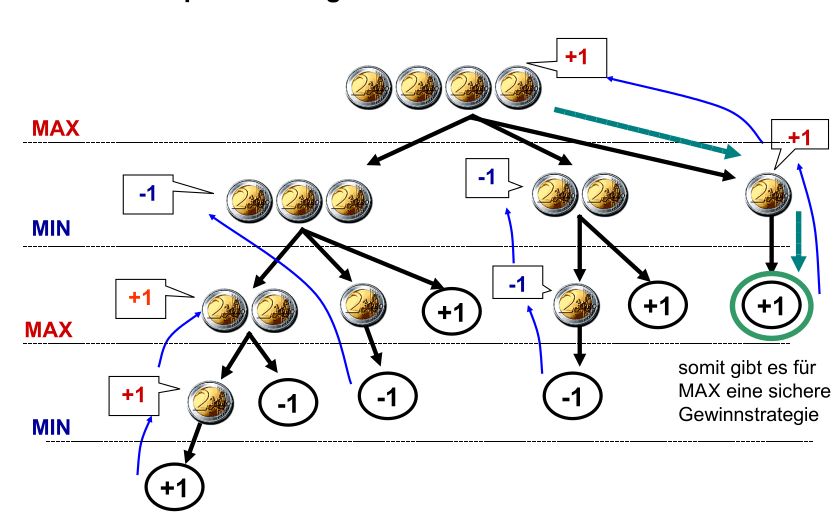
\includegraphics[width=0.8\textwidth]{figures/kap4/minmax-nimm.png}
    \caption{Bottom-up Bewertung der Knoten aus der Sicht von MAX}
    \label{fig:minmax-nimm-example}
\end{figure}

\subsection{Eigenschaften des MiniMax-Algorithmus}

Der Algorithmus ist vollst�ndig, wenn der Suchbaum endlich ist, und ist optimal, wenn gegen einen optimalen Spieler gespielt wird. Der Algorithmus hat ein Zeitbedarf von \(O(b^m)\) miz Suchtiefe \(m\) und Verzweigungsfaktor \(b\) und hat ein Platzbedarf von \(O(b*m)\). 

Dieser Algorithmus kann modifiziert werden, indem man die Tiefe des Baumes begrenzt (nur ein paar Runden vorausschaut) und den Nutzen einer Position mit einer guten Bewertungsfunktion absch�tzt.

\subsection{Verbesserung des MiniMax-Algorithmus durch Pruning}

Pruning, auch bekannt als \(\alpha\beta\)-Search oder \(\alpha\beta\)-Pruning, ist eine Idee, um die Effizienz des Minimax-Algorithmus zu verbessern, indem fr�hzeitig erkannt wird, welchem Zweig des Suchbaums nicht gefolgt werden muss.

Unter der Annahme, dass MIN und MAX jeweils den f�r sie optimalen Weg w�hlen, ist es m�glich fr�hzeitig zu erkennen, welche Verzweigungen des Suchbaums das Ergebnis nicht beeinflussen und daher nicht berechnet werden m�ssen. Unter Verwendung des Nimm-Beispiels k�nnen Pfade geschnitten werden, die ein schlechteres Ergebnis liefern als bereits erkundete Pfade.

\begin{figure}[H]
    \centering
    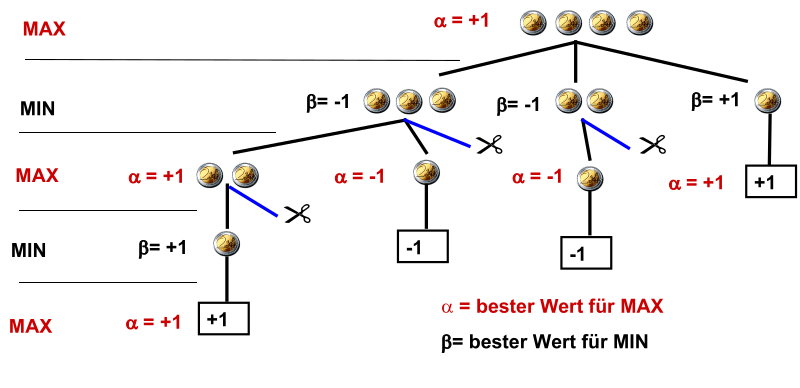
\includegraphics[width=0.8\textwidth]{figures/kap4/minxmax-pruning.png}
    \caption{Beschneiden des MinMax-Nimm-Beispiels}
    \label{fig:minmax-pruning-example}
\end{figure}

\subsection{Komplexit�t von MiniMax-Pruning}

Im schlimmsten Fall, wenn die Knoten in einer ung�nstigen Reihenfolge sind, dann ist es dasselbe wie bei einem normalen MiniMax. Im besten Fall k�nnte man die Mindestanzahl an Positionen berechnen lassen. Dies kann erreicht werden, indem die Reihenfolge der Bewegungen basierend auf der Effizienz der Bewegung neu geordnet wird. Zum Beispiel ist beim Schach das Schlagen einer Figur mit einem Turm oft vorteilhaft und sollte zuerst sequenziert werden.

\subsection{MiniMax in Spielen mit Zuf�lligkeit}

Die Zuf�lligkeit wird unter Verwendung zus�tzlicher Knoten im Suchbaum gehandhabt. F�r die Bewertung erh�lt jeder Zweig der Zufallsknoten den Durchschnitt aller m�glichen Zufallsergebnisse. 

\begin{figure}[H]
    \centering
    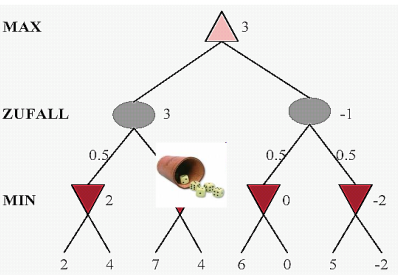
\includegraphics[width=0.6\textwidth]{figures/kap4/minmax-random.png}
    \caption{Zus�tzlicher Zufallknoten mit Mittelwert-Bewertung}
    \label{fig:minmax-random-example}
\end{figure}

\section{Monte Carlo Tree-Search}

In gro�en Suchr�umen wie Schach oder Go ist der MiniMax-Algorithmus weniger geeignet, da zu viele Knoten erweitert werden m�ssten. Die Idee von Mote Carlo Tree Search (MCTS) ist, dass ein Suchbaum wie in MiniMax ebenfalls generiert wird, aber anstatt alle m�glichen Positionen zu erweitern, werden die Z�ge durch zuf�llige Z�ge �ber (sehr) viele Spiele erweitert.

\subsection{Ablauf des MCTS-Algorithmus}

Die folgenden Schritte werden wiederholt durchgef�hrt:-

Die folgenden Schritte werden so lange wiederholt, bis der Alhorithmus zum Abbrechen aufgefordert wird:

\begin{enumerate}
    \item \textbf{Selection}. Max beginnt bei der Wurzel, um einen g�nstigen Zug zu w�hlen. Wenn noch keine Informationen vorliegen, wird ein zuf�lliger Zug gew�hlt.
    \item \textbf{Expansion}. Wenn ein ausgew�hlter untergeordneter Knoten nicht der Endzustand ist, werden alle m�glichen Nachfolger hinzugef�gt und einer ausgew�hlt.
    \item \textbf{Simulation}. Ab dem ausgew�hlten Knotenpunkt wird das Spiel gespielt, bis es mit einem Sieg, einer Niederlage oder einem Remis endet.
    \item \textbf{Backpropagation}. �bertrage die Ergebnisse des Spiels von den Endknoten zur�ck zum Wurzel und aktualisiere die Knoten auf dem Pfad.
\end{enumerate}

Der daraus resultierende Suchbaum sieht in etwa so aus wie in der Abbildung~\ref{fig:monte-carlo-tree-example}.

\begin{figure}[H]
    \centering
    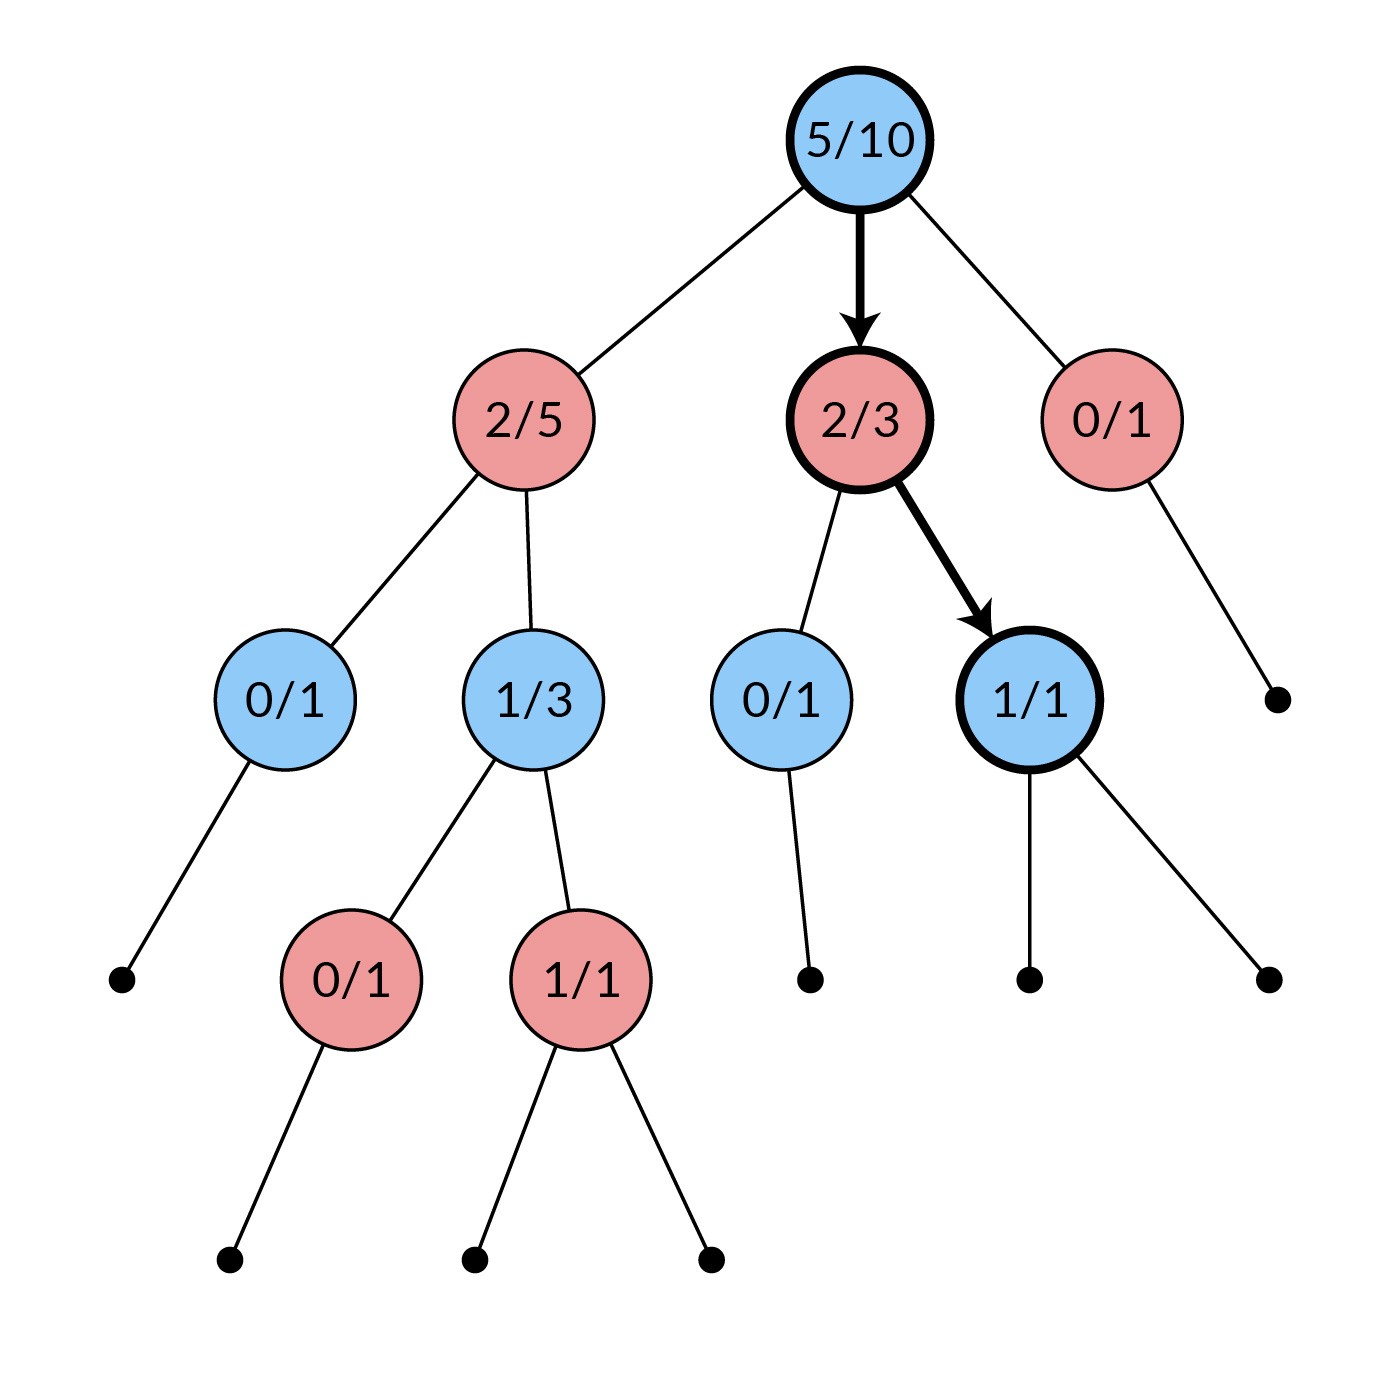
\includegraphics[width=0.65\textwidth]{figures/kap4/monte-carlo-tree-example.jpeg}
    \caption{Beispiel f�r einen Monte-Carlo-Suchbaum}
    \label{fig:monte-carlo-tree-example}
\end{figure}

Jeder Knoten hat einen Wert von \(Siege/Spiele\). Mit diesem Wert kann der beste Knoten basierend auf einem hohen Verh�ltnis von Gewinnen zu gespielten Spielen ausgew�hlt werden.
\chapter{Constraints}

Bei vielen Problemen gibt es Abh�ngigkeiten in den L�sungskomponenten. Es gibt zum Beispiel F�lle, in denen wenn X den Wert A hat dann hat Y den Wert B. Oder wie im Spiel Sudoku kann dieselbe Zahl nicht zweimal in derselben Reihe oder Diagonale vorkommen. Probleme, bei denen Constraints eine Rolle spielen, und wie sie gel�st werden k�nnen, werden in diesem Kapitel behandelt.

\section{L�sen von Constrain-Problemen}

\paragraph{Allgemeines Constraint Solving Problem}

Bei einer gegebenen Menge von Variablen innerhalb eines bestimmten Wertebereichs und einer Menge von Beschr�nkungen erlaubter Kombinationen der Variablenwerte wird nach einer konkreten Anordnung der Variablen gesucht, die alle Beschr�nkungen erf�llen kann.

\paragraph{Constraint Solving Problem als Suche}

Solche Probleme k�nnen als Suchproblem dargestellt werden, wobei:
\begin{itemize}
    \item \textbf{Suchraum:} Menge von Variablen und derren Dom�nen
    \item \textbf{Anfangszustand:} Alle Variables sind noch unbelegt
    \item \textbf{Zielzustand:} alle Variablen belegt und Constraints erf�llt
    \item \textbf{Zieltest:} �berpr�fe, ob alle Variablen die Constraints erf�llen
\end{itemize}

\subsection{Ans�tze z�r L�sung von Constraint Solving Problemen}

\paragraph{Ansatz 1: Generiere und Teste}

Generiere Kombinationen von Werten f�r die Variablen basierend auf ihren Dom�nen und teste, ob die Bedingungen erf�llt sind. Wiederhole so oft wie n�tig.


\begin{table}[H]
    \centering
    \begin{tabular}{|l|l|l|l|}
    \hline
    \(x_1\) & \(x_2\) & \(x_3\) & \textbf{Test} \\ \hline
    1           & 1           & 1           & nein          \\ \hline
    1           & 1           & 2           & nein          \\ \hline
    1           & 2           & 1           & nein          \\ \hline
    1           & 2           & 2           & nein          \\ \hline
    2           & 1           & 1           & nein          \\ \hline
    2           & 1           & 2           & nein          \\ \hline
    2           & 2           & 1           & ja            \\ \hline
    \end{tabular}
    \caption{\label{tab:generate-and-test} Ergebnis des Generierens und Testens}
\end{table}

\paragraph{Ansatz 2: Tiefensuche mit Backtracking}

Die Werte f�r die Variablen werden systematisch generiert, um nicht alle m�glichen Kombinationen generieren zu m�ssen.

\begin{table}[H]
    \centering
    \begin{tabular}{|l|l|l|l|}
    \hline
    \(x_1\) & \(x_2\) & \(x_3\) & \textbf{Test} \\ \hline
    1           & 1           & 1           & nein          \\ \hline
    1           & 1           & 2           & nein          \\ \hline
    1           & 2           & 2           & nein          \\ \hline
    1           & 2           & 1           & nein          \\ \hline
    2           & 2           & 1           & ja            \\ \hline
    \end{tabular}
    \caption{\label{tab:deepsearch-and-backtracking} Ergebnis von Tiefensuche und Backtracking}
\end{table}

Durch den Einsatz von Heuristiken und anwendungsspezifischen Merkmalen kann die L�sung von Constraint-Problemen effizienter gestaltet werden. Unter Verwendung von Constraints kann der Zustandsraum umstrukturiert werden, um die Constraints zum leichteren L�sen des Problems auszunutzen.

\subsection{Optimierung der L�sung von Constraint Problemen}

Die folgenden Optimierungen lassen sich anhand eines konkreten Beispiels besser erkl�ren. Ein Beispiel f�r ein Problem mit Cosntraints ist die Einf�rbung von Staaten in Australien mit drei Farben, so dass benachbarte Staaten niemals dieselbe Farbe haben.

\begin{figure}[H]
    \centering
    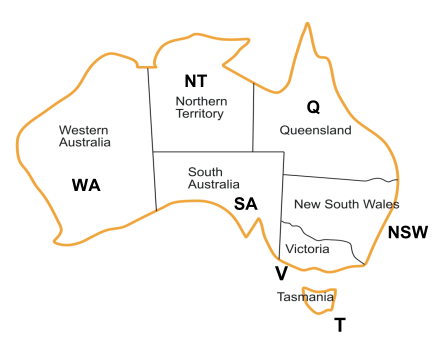
\includegraphics[width=0.6\textwidth]{figures/kap5/australia-map.png}
    \caption{Karte der Staaten von Australien}
    \label{fig:constraints-australia-states}
\end{figure}

\paragraph{Anwendung von Constraint Netzen}

Ein Netz kann erstellt werden, wenn Probleme bin�re Beschr�nkungen haben. Die Variablen sind die Knoten und die Kanten verbinden die Knoten mit Nebenbedingungen.

\begin{figure}[H]
    \centering
    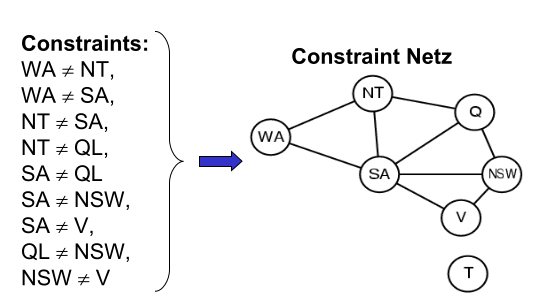
\includegraphics[width=0.6\textwidth]{figures/kap5/australia-constraint-net.png}
    \caption{Constraints-Netz}
    \label{fig:constraint-net-australia}
\end{figure}

Das Constraints Netz kann in Heuristiken verwendet werden, um die Nutzung der Tiefensuche mit Backtracking zu verbessern.

\paragraph{Abalauf von Tiefensuche mit Backtracking zur L�sung von Constraint Problemen}

Mit Hilfe einer \textbf{Degree Heuristik}, bei der mit der Variable begonnen wird, die die meisten Constraints aufweist, kann die Suche optimiert werden. Based on the Constraint Netz in Abb.~\ref{fig:constraint-net-australia}, k�nnen wir sehen, dass SA die meisten Einschr�nkungen hat und die Suche damit beginnen sollte. Danach wird die Suche wie eine typische Tiefensuche (siehe Abschnitt~\ref{section:depth-search-backtracking}) fortgesetzt:-

\begin{enumerate}
    \item In jedem Schritt wird einer Variablen ein Wert zugeordnet.
    \item Wenn die Variable nicht mehr so erweitert werden kann, dass sie den Beschr�nkungen entspricht, wird ein Backtracking durchgef�hrt.
\end{enumerate}

Eine weitere Heuristik, die verwendet werden kann, ist die Minimum-Remaining-Value-Heuristik. 

\section{Vertiefungsprojekt: N-Damen Problem mittels Choco-Solver}

Um besser zu verstehen, wie Constraint-Probleme mit konventionellen Programmiersprachen gel�st werden, wurde das N-Queen-Problem in Java implementiert.

\begin{figure}[H]
    \centering
    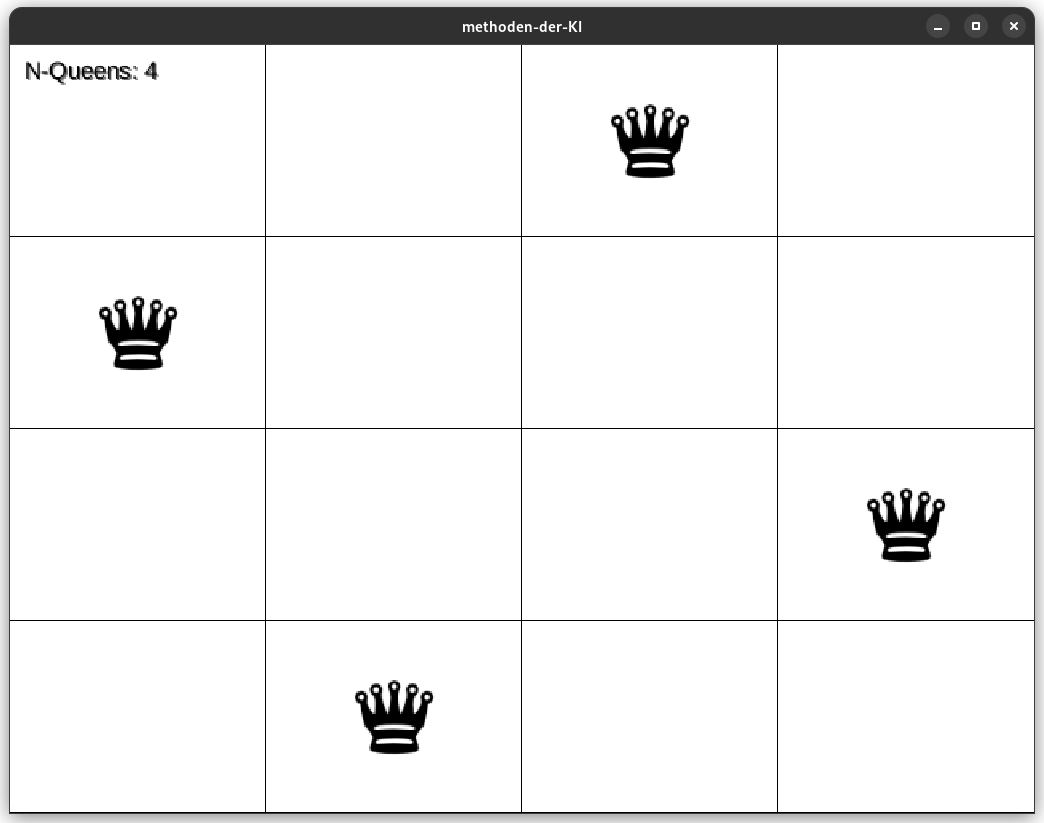
\includegraphics[width=0.8\textwidth]{figures/kap5/n-queens-impl.png}
    \caption{N-Damen Implementierung mit n=4}
    \label{fig:impl-n-damen}
\end{figure}

In diesem Programm wird das n-Damen-Problem f�r n=4 bis 27 unter Verwendung von Constraints gel�st. In diesem Programm w�rde das Dr�cken der Aufw�rts- und Abw�rtspfeiltasten den Wert von N entsprechend erh�hen oder verringern. Das Gitter aktualisiert sich dann selbst, um n x n beizubehalten, und der Choco-Cosntraintssl�ser wird jedes Mal verwendet, wenn sich n �ndert, um eine L�sung zu generieren. Das Programm funktioniert f�r Werte von n von 4 bis 27, aber da die Gr��e des Damenbildes nicht skaliert, ist es schwer zu sehen, wo genau eine Dame nach n=18 platziert wird.

Die Tastensteuerungen wie folgt:
\begin{itemize}
    \item \textbf{Up Arrow Key:} Erh�ht den Wert von N.
    \item \textbf{Down Arrow Key:} Verringert den Wert von N.
    \item \textbf{Escape-Taste:} Geht zur�ck zum Start-Screen.
\end{itemize}

Der relevante Code f�r das Programm befindet sich in den folgenden Packages:
\begin{itemize}
    \item \textbf{de.augsburg.hs.methoden.ki.algorithms.constraints:} Implementierung der Constraints mit Choco-Solver.
    \item \textbf{de.augsburg.hs.methoden.ki.screens.minmax} Klasse f�r den N-Queen-Screen.
    \item \textbf{de.augsburg.hs.methoden.ki.actors.nqueens:} Klassen f�r die Darstellung der Damen.
\end{itemize}

\input{kapitel/5/kap_5.3.tex}

\input{kapitel/5/kap_5.4.tex}
\chapter{Wissensbasierte Systeme}

Wissensbasierte Systeme verwenden wissensbasierte Informationsverarbeitung, um L�sungen f�r Probleme zu berechnen. Diese Art der Informationsverarbeitung ist ein Paradigma, das eine strikte Trennung von Wissen und den zur L�sung des Problems erforderlichen Verarbeitungsmechanismen erfordert.

In einem klassischen System besteht ein Programm aus Programmen und Algorithmen. Ein wissensbasiertes System hingegen besteht aus symbolisch dargestelltem Wissen und Verarbeitungsmechanismen, um dieses Wissen zur Probleml�sung zu nutzen.

\begin{figure}[H]
    \centering
    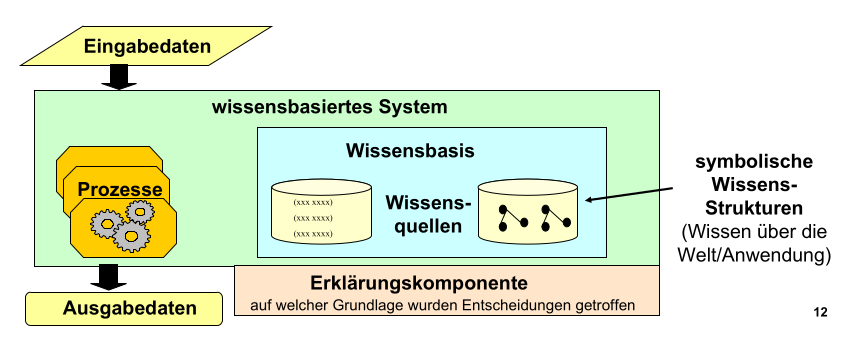
\includegraphics[width=\textwidth]{figures/kap6/anatomie-wbs.png}
    \caption{�berblick �ber ein wissensbasiertes System}
    \label{fig:overview-wbs}
\end{figure}

\section{Wissensdarstellung in wissensbasierten Systemen}

Wissensbasierte Informationsverarbeitung basiert auf der Vorstellung, dass viele Probleme nur l�sbar sind, wenn man Erfahrung mit dem Problem und den L�sungsm�glichkeiten daf�r hat. Dies wirft die Frage auf: Wie stellen wir Wissen so dar, dass es von Computern verstanden und zur Probleml�sung verwendet werden kann?

Wissen wird dabei als Klassen, Kategorien und Konzepte mit Hierarchien, Zusammensetzungen und Klassifikationen dargestellt. Dies ist eine ontologische Erfassung einer Anwendungsdom�ne bekannt. Diese Art der Datenmodellierung l�sst sich am besten mit einer Mindmap vergleichen (siehe Abb.~\ref{fig:mind-map-example}).

\begin{figure}[H]
    \centering
    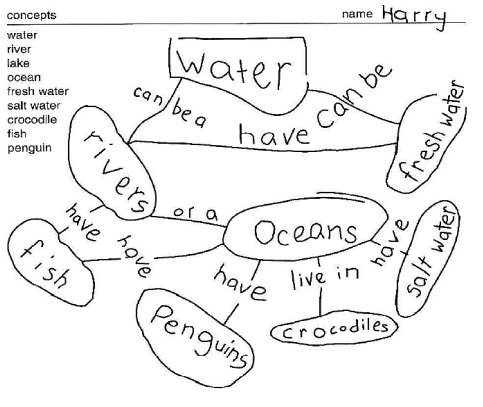
\includegraphics[width=0.52\textwidth]{figures/kap6/mind-map.png}
    \caption{Beispiel einer Mindmap von einem Grundsch�ler}
    \label{fig:mind-map-example}
\end{figure}

Diese Klassen, Kategorien und Konzepte werden letztlich in der Implementierung durch programmtypische Datenstrukturen wie Objekt-Arrays und Pointer abstrahiert (Abb.~\ref{fig:knowledge-darsetllung-ebenen}).

\begin{figure}[H]
    \centering
    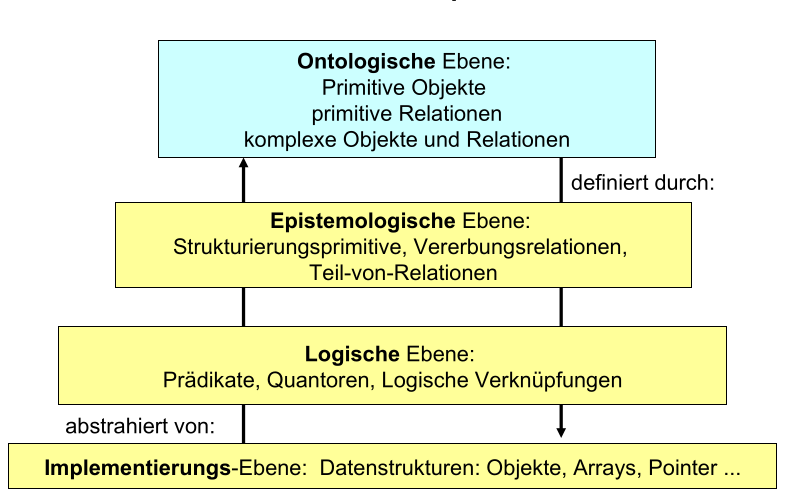
\includegraphics[width=0.8\textwidth]{figures/kap6/ebenen-wissendarstellung.png}
    \caption{Ebenen der Wissensrepr�sentation}
    \label{fig:knowledge-darsetllung-ebenen}
\end{figure}

Es gibt viele M�glichkeiten, Wissen explizit darzustellen. Eine Anwendung kann logikbasierte Ans�tze wie Fakten und Regeln verwenden. Andere k�nnen Rahmen und F�lle oder strukturierte Vererbungsnetze �hnlich objektorientierter Modelle verwenden.

\section{Schnittstelle zur Interaktion mit einem Wissenbassierten System}

Damit ein Benutzer mit einem wissensbasierten System interagieren kann, muss eine Schnittstelle vorhanden sein, die mindestens die folgenden Funktionen ausf�hren kann:

\begin{itemize}
    \item \textbf{Tell(WBS, knowledge-item):} F�ge dem System neues Wissen hinzu. z.B: "Die Welt ist Rund"
    \item \textbf{Ask(WBS, question):} Anfrage stellen. z.B: ist die Welt eine Kugel?
\end{itemize}

Allein durch die Verwendung dieser beiden Funktionen kann ein wissensbasiertes System verwendet werden, um Probleme innerhalb seiner Wissensbasis zu l�sen.

\section{Ans�tze zur Wissensverarbeitung}

Eine wichtige Komponente eines wissensbasierten Systems ist die Inferenzmaschine, die verwendet wird, um unsere Antworten auf Fragen zu finden. Es gibt viele Ans�tze f�r die Implementierung einer solchen Maschine zur Verarbeitung von vorhandenem Wissen.

\paragraph{Prinzip der Wissensabstraktion}

Diese Methode wird als induktive Inferenz bezeichnet: Ableitung allgemeiner Aussagen aus Spezialf�llen. z.B:

\begin{itemize}
    \item Beobachtung: Studenten Hans und Fritz haben ein Laptop
    \item Schlussfolgerung: Alle Studenten haben Laptops
\end{itemize}

\paragraph{Prinzip von Wissen �ber Wissensintegrit�t}

Diese Methode wird als deduktive Inferenz bezeichnet: Durch Erkennung von Regeln und Invarianzen aus formalen Beschreibungen wird explizites Wissen explizit gemacht. z.B:

\begin{itemize}
    \item Beobachtung: Aussage A ist wahr und Aussage B ist wahr.
    \item Schlussfolgerung: Auch die Aussage A oder B ist wahr.
\end{itemize}

\paragraph{Prinzip von Wissen �ber Kausalzusammenh�nge}

Diese Methode wird als abduktive Inferenz bezeichnet: Die Ursachen werden aus Beobachtungen abgeleitet: A ist der Grund daf�r, dass B passiert ist, wenn also B beobachtet wird, ist A passiert. z.B:

\begin{itemize}
    \item Beobachtung: Licht ist an.
    \item Schlussfolgerung: Lichtschalter ist auf Position ``Ein''.
\end{itemize}

\paragraph{Wissen �ber Analogien}

Diese Methode wird als analoge Inferenz bezeichnet: Neue Erkenntnisse werden aus bereits bekannten abgeleitet. z.B:

\begin{itemize}
    \item Beobachtung: durch ein dickes Rohr kann viel Wasser flie�en.
    \item Schlussfolgerung: durch ein dickes Kabel kann viel Strom flie�en.
\end{itemize}

\paragraph{Prinzip der Verwendung von empirischem Wissen}

Diese Methode wird als probabilistische Inferenz bezeichnet: Schlussfolgerung, dass eine Wirkung eintritt, basierend auf der Wahrscheinlichkeit, dass sie aufgrund der Situation eintritt. z.B:

\begin{itemize}
    \item Wenn 100 Personen im Raum sind, kann man davon ausgehen, dass mindestens zwei von ihnen denselben Geburtstag haben.
\end{itemize}

\paragraph{Prinzip der Verwendung von unscharfem Wissen}

Diese Methode wird als Fuzzy-Inferenz bezeichnet: Schlussfolgerungen auf der Grundlage der Wahrscheinlichkeit, dass ein Objekt zu einer Menge geh�rt. z.B:

\begin{itemize}
    \item Hans ist vierzig Jahre alt. Alte Menschen sind weise.
    \item Zugeh�rigkiet Hans zur Menge der jungen Menschen: 0.6
    \item Zugeh�rigkiet Hans zur Menge der alten Menschen: 0.4
    \item Ask: Ist Hans Weise? Antwort: Na ja, geht so
\end{itemize}

\section{Aufgaben beim Entwurf eines Wissenbassierten Systems}

Es ist es wichtig, von Anfang an herauszufinden, welche Arten von Wissen es zu erwerben gilt und wie diese repr�sentiert und gespeichert werden. Daneben muss auch entschieden werden, welche Inferenzmechanismen verwendet werden sollen.

Dann stellt sich die Frage, wie die Wissensbasis gef�llt werden soll. Dazu gibt es einfache Methoden, z. B. indem man einen Experten dazu bringt, sein Wissen mit einem Texteditor, einem Formular oder einem Mikrofon einzugeben. Es gibt aber auch komplexere Ans�tze wie die Entwicklung einer Schnittstelle zur Umwandlung von Datenbankinhalten in ein Format, das von einem wissensbasierten System verarbeitet werden kann, oder die Extraktion neuen Wissens mit Hilfe k�nstlicher neuronaler Netze. 

\section{Vertiefung: The Bitter Lesson}

In dem kurzen Essay von Richard Sutton, einem kanadischen Informatiker, diskutiert er den seiner Meinung nach gr��ten Fehler der KI-Forschung der letzten 70 Jahre. Er argumentiert, dass die KI-Forschung durch einen zu starken Fokus auf die Verwendung von Ans�tzen des ``menschlichen Wissens'' anstelle der Verwendung von Rechenleistung behindert wurde.

Als Beispiel verwies er auf das Jahr 1997, als Kasparov, Schachweltmeister, von einem Computer besiegt wurde, der Deep Search mit spezieller Hard- und Software verwendete, anstatt das menschliche Verst�ndnis der besonderen Natur des Schachs zu nutzen. Diese Methode wurde von der Mehrheit der Computerschachforscher abgelehnt, die entt�uscht waren, dass das System keine Methoden verwendete, die auf menschlichem Input basierten, um zu gewinnen.

�hnliche Situationen gab es bei der Entwicklung von Computer Go, Spracherkennung und Computer Vision. Dabei kamen zun�chst solche Ans�tze: die Besonderheiten des Spiels bei Go, die Kenntnis von W�rtern und Ph�nomenen f�r die Spracherkennung oder die Suche nach Kanten und Zylindern im Computer Vision. Am Ende wurde all dies jedoch zugunsten neuerer Methoden verworfen, die sich die rohe Rechenleistung zunutze machen, die aufgrund des Mooresschen Gesetzes zur Verf�gung gestellt wurde.

Die bitteren Lehren laut Richard Sutton sind, dass die Leistungsf�higkeit von Allzweckmethoden, die mit zunehmender Rechenleistung weiter skalieren, nicht untersch�tzt werden sollte und dass sich die KI-Forschung darauf konzentrieren sollte, KI-Agenten zu erm�glichen, herauszufinden, wie sie die Au�enwelt verstehen k�nnen. und der KI keine bestimmte Denkweise aufzuzwingen.
% \include{einleitung}
% \include{unternehmen}

% \include{projekt_a}
% \include{stellungnahme}

%\include{beispiele}   % Beispiele
%\include{beispiele2}     % Beispiele2

%\chapter*{Hinweis Literatur}
Beachten Sie, dass auch in einem Praxisbericht alle verwendeten Quellen eindeutig gekennzeichnet sein m�ssen. Insbesondere m�ssen Sie auch Bildquellen angeben (sofern Sie die Bilder nicht selbst aufgenommen/erstellt haben). Ebenso muss die Verwendung von Inhalten aus Firmenpr�sentationen angegeben werden. Der Bezug der Textstelle zur Quelle muss eindeutig sein.

Vermeiden Sie die Angabe von Webseiten als Quellen. Wenn Sie diese dennoch verwenden wollen, achten Sie auf eine Angabe der URL mit Abrufdatum und erg�nzen Sie die Quelle falls m�glich mit Autor und Titel.


%% ++++++++++++++++++++++++++++++++++++++++++
%% Anhang
%% ++++++++++++++++++++++++++++++++++++++++++

%\appendix
%\include{anhang_a}
%\include{anhang_b}

%\ifnotonesideelse{\cleardoublepage}{}

%% ++++++++++++++++++++++++++++++++++++++++++
%% Literatur
%% ++++++++++++++++++++++++++++++++++++++++++
\addcontentsline{toc}{chapter}{\bibname}
%  mit dem Befehl \nocite werden auch nicht zitierte Referenzen abgedruckt 
% (normalerweise nicht erwünscht)
% \nocite{*}
\bibliographystyle{rialpha}
%Einbinden Bibtexdatei - Direkt aus JabRef generiert
\bibliography{literatur}
%% ++++++++++++++++++++++++++++++++++++++++++
%% Index (optional)
%% ++++++++++++++++++++++++++++++++++++++++++
%\ifnotdraft{
%\addcontentsline{toc}{chapter}{Index}
%\printindex            % Index, Stichwortverzeichnis
%}
\end{document}
